\documentclass[tikz,border=0pt]{standalone}
\usepackage{climbingguide}

\begin{document}
\directlua{
    cg.set_zone("ZONA BOQUEIRÃO")
    cg.set_sector("MOCOZADO")
    cg.register_route(1, "Via Alfa", "V", "15m", "2+2", "Setter A")
    cg.register_route(2, "Via Beta", "VIb", "20m", "4+2", "Setter B")
    
    cg.set_sector("MOCOZINHO")
    cg.register_route(3, "Via Gamma", "VIIa", "25m", "6+2", "Setter C")
    cg.register_route(4, "Via Delta", "VIIIa", "30m", "8+2", "Setter D")
    cg.register_route(5, "Via Epsilon", "Proj.", "35m", "Mista", "Setter E")

    cg.set_zone("ZONA SERRA NEGRA")
    cg.set_sector("PAREDÃO ALTO")
    cg.register_route(6, "Via Zeta", "IVsup", "18m", "3+2", "Setter F")
    cg.register_route(7, "Via Eta", "VIa", "22m", "5+2", "Setter G")
    cg.register_route(8, "Via Theta", "IXb", "40m", "12+2", "Setter H")
}

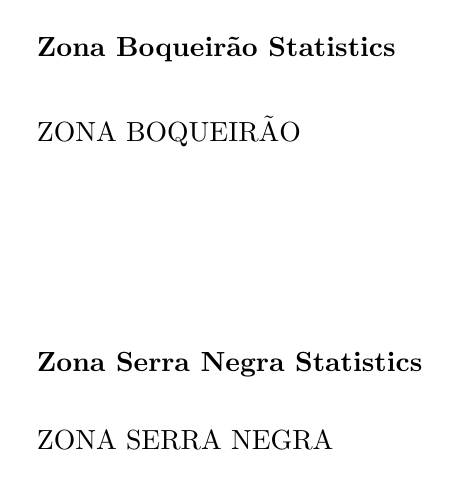
\begin{tikzpicture}
    \node[anchor=north west] at (0,3) {\textbf{Zona Boqueirão Statistics}};
    \node[anchor=north west] at (0,2) {\CGZoneStats{ZONA BOQUEIRÃO}};
    
    \node[anchor=north west] at (0,-1) {\textbf{Zona Serra Negra Statistics}};
    \node[anchor=north west] at (0,-2) {\CGZoneStats{ZONA SERRA NEGRA}};
\end{tikzpicture}
\end{document}
